\documentclass[12pt]{article}
\usepackage{fullpage}
\usepackage[margin=1in]{geometry}
\usepackage[stable]{footmisc}
\usepackage{graphicx}
\usepackage{amssymb}
\usepackage{IEEEtrantools}
\usepackage{lineno}
\usepackage{amsmath}
\usepackage{epstopdf}
\usepackage{parskip}
\usepackage{authblk}
\usepackage[authoryear]{natbib}
%\setlength{\parskip}{20pt}
\linespread{1.6}
\date{}

\DeclareGraphicsRule{.tif}{png}{.png}{`convert #1 `dirname #1`/`basename #1 .tif`.png}


%%	math short-cuts
\def \ve{\varepsilon}	% epsilon used for metabolic rate
\def \la{\lambda}	% lambda
\newcommand{\eref}[1]{(\ref{#1})}

%%	new commands for referencing figures and tables and sections
\newcommand{\fref}[1]{Figure~\ref{#1}}	% inline figure ref
\newcommand{\fpref}[1]{Fig.~\ref{#1}}	% parenthetical figure ref
\newcommand{\tref}[1]{Table~\ref{#1}}	% table ref
\newcommand{\sref}[1]{Section~\ref{#1}}	% table ref
%\linenumbers

\title{\Large \textbf{Integrated MERA: combining MERA I, II, and III}}

\author{Jade, Nov 10}

\begin{document}
\maketitle
\raggedright
\large
\setlength{\parindent}{15pt}
Here I will merge 1) resource allocation among species and individuals as is described by MERA I \& II and 2) resource acquisition by all species from the environment as is described by MERA III, and develop an integrated model of MERA. In the solution we can see that some of the properties of I, II and III are retained but there are also new properties emerging: not only $\theta$ and $D_r$, the intrinsic growth rate $r$ of the species also affects its steady state abundance.

\section{Quick recap of MERA II}
First let's recall the generalized $W_{total}$ derived from MERA II (June 8 write up):
 \begin{equation}
 \begin{split}
 \mbox{log }W_{total} =  \mbox{log }W_{across}+\sum^{S_0}_i D_{r,i} \mbox{log }W_{within,i}\\
 =  - R_{0}\sum^{S_0}_i P_i\mbox{log } P_i - \sum^{S_0}_i D_{r,i} R_i  \sum^{N_i}_j p_{ij} \mbox{log } p_{ij}
 \end{split}
\end{equation}

Where $P_i = R_i/R_0$ is the relative resource abundance of species $i$ in the community and $p_{ij}= r_j/R_i$ is the relative resource abundance of individual $j$ in species $i$.  Also $W_{grouping}$ is left out since the definition of demographic group is trivial here (in MERA II an individual can get any amount of resource). For each species $i$ maximizing $\sum^{N_i}_j p_{ij} \mbox{log } p_{ij}$ yields a uniform distribution for $p_{ij}$:
 \begin{equation}
p_{ij} = \frac{1}{N_i}
\end{equation}
Substituting Eq. 2 into Eq. 1 we get
 \begin{equation}
 \begin{split}
 \mbox{log }W_{total} =  - R_{0}\sum^{S_0}_i P_i (\mbox{log } P_i + D_{r,i} \mbox{log } N_i)
\end{split}
\end{equation}
 Then $ \mbox{log }W_{total}$ is maximized respect to $P_i$ subject to the normalization constraint ($\sum^{S_0}_i P_i = 1$), which gives
  \begin{equation}
 \begin{split}
 P_i \propto N_i^{D_{r,i}}\\
 =>  R_i = R_0 \frac{N_i^{D_{r,i}}}{\sum^{S_0}_j {N_j}^{D_{r,j}}}
\end{split}
\end{equation}
A problem of this solution is that, there is no upper limit to how many resources a species can get. Specifically, if $R_0$ is big enough, $R_i$ can be big even if $N_i$ is small, generating unrealistically huge growth. Below I will show how MERA III helps solve this problem.

\section{Combine II and III: allocation with upper limits for species boxes}
In MERA III, we have introduced a resource acquisition procedure where resource in the environment are randomly allocated to resource acquisition activities of the species, the magnitude of which is regulated by the species current abundance $N$ and intrinsic growth rate $r$ (from here on I will call this value the resource capacity of the species, given its $r$ and $N$ at the time). The allocation stopped at the community level, not considering distribution of the resource among or within species. Here I will introduce an integrated procedure to allocate resources in the environment 1) to species resource capacity boxes (regulated by $N$ and $r$), then 2) within each species to individuals. 

*My original thought was to use MERA III to determine the resource constraint for the whole community, then apply MERA I or II to get species and individual level distributions. This turns out not to work as expected since although it can make sure the total resource capacity for the community is not surpassed, it does not guarantee for every single species not to surpass its resource capacity. Therefore the resource capacity boxes cannot be lumped  and species level allocation has to happen simultaneously with acquisition. Under this framework, the concept for community-level resource constraint is not necessary any more. *

graph demo

$C_i$ is the resource capacity for species $i$:
 \begin{equation}
C_i = (r_i+1)N_i \theta_i
\end{equation}
$R_i$ is the actual amount of resources allocated to species $i$. 

The total number of microstates for a given species-level resource distribution $R_i$ ($i$ in 1, ..., $S_0$) is
 \begin{equation}
 \begin{split}
W_{total}(R_{1,..., S_0})  =  \prod_i^{S_0}W_{acquisition,i} \times W_{across} \times\prod_i^{S_0}W_{within,i} ^{D_{r,i}}
\end{split}
\end{equation}
Where $W_{acquisition,i}$ is the number of ways to select $R_i$ out of $C_i$ empty spots in the species capacity pool to be filled each with a unit of resource. 
 \begin{equation}
 \begin{split}
W_{acquisition,i} = \frac{C_i!}{R_i! (C_i-R_i)!}
\end{split}
\end{equation}
A spot in $C_i$ can be taken as a resource acquisition activity which can acquire one unit of resource if successful, or zero resource if failed. Therefore $R_i/C_i$ can be taken as the success rate in resource acquisition. 

$W_{across}$ is the number of ways to allocate the total resource in the environment into species boxes ($R_i$s) as well as the ``unused'' box (which contains all resources that are not utilized by any species).
 \begin{equation}
 \begin{split}
W_{across} = \frac{R_0!}{\prod_i^{S_0}R_i! \times (R_0-\sum_i^{S_0}R_i)!}
\end{split}
\end{equation}
$W_{within,i}$ is the number of ways to allocate $R_i$ resource units to $N_i$ individuals:
 \begin{equation}
 \begin{split}
W_{within,i} = \frac{R_i!}{\prod_j^{N_i}r_{ij}! }
\end{split}
\end{equation}

 Substituting Eqs. 7-9 into Eq. 6 and log-transform:
  \begin{equation}
 \begin{split}
 \mbox{log }W_{total} = \sum^{S_0}_i [C_i \mbox{log } C_i - R_i \mbox{log } R_i - (C_i-R_i) \mbox{log } (C_i-R_i)] \\
 + R_0 \mbox{log } R_0 - \sum^{S_0}_i R_i\mbox{log } R_i - (R_0-\sum_i^{S_0}R_i) \mbox{log }(R_0-\sum_i^{S_0}R_i) \\
 - \sum^{S_0}_i R_i D_{r,i} \mbox{log } N_i\\
 = R_0 \mbox{log } R_0 + \sum^{S_0}_i C_i \mbox{log } C_i \\
 - \sum^{S_0}_i [2 R_i\mbox{log } R_i + (C_i-R_i) \mbox{log } (C_i-R_i)+ R_i D_{r,i} \mbox{log } N_i]\\
 - (R_0-\sum_i^{S_0}R_i) \mbox{log }(R_0-\sum_i^{S_0}R_i)
\end{split}
\end{equation}
Notice that in Eq. 10 $W_{within,i}$ is already maximized:
  \begin{equation}
max ( \mbox{log } W_{within,i}  )=  R_i \mbox{log } N_i
\end{equation}

Maximizing $ \mbox{log }W_{total}$ (no constraint) yields
  \begin{equation}
R_i^2 = (C_i-R_i)(R_0 -\sum_i^{S_0}R_i) N_i ^{D_{r,i}}
\end{equation}

Easy to see that the one species case with $D_{r,i}=0$ (see discussion) gives exactly the same solution as the previous MERA III (write-up Oct 16). For an arbitrary set of $N_i$s $R_i$ has to numerically solved with $S_0$ simultaneous equations (Eq. 12 for all species). At steady state however, since the resource allocated to each species happen to provide for exactly the current abundance, or  $\hat{R_i} = \theta_i \hat{N_i}$, we have
  \begin{equation}
   \begin{split}
(\theta_i \hat{N_i})^2 =\hat{R_i}^2=  [(r_i+1)\theta_i \hat{N_i} -\theta_i \hat{N_i}](R_0 -\sum_i^{S_0}\theta_i \hat{N_i}) \hat{N_i} ^{D_{r,i}}
= r_i \theta_i \hat{N_i} R_u \hat{N_i} ^{D_{r,i}} \\
=> \hat{N_i} = (\frac{\theta_i}{r_i R_u})^{\frac{1}{D_{r,i}-1}}\hskip 5cm
\end{split}
\end{equation}
where $R_u = R_0 -\sum_i^{S_0}\theta_i \hat{N_i}$ is the amount of unused resource at steady state. From Eq. 13 we can see that when all species have the same intrinsic growth rate $r$, the steady state solution is the same as MERA I and II ($ \hat{N_i} \propto  \theta_i ^{\frac{1}{D_{r,i}-1}}$). However, when $r_i$ varies from species to species, the steady state solution is different. Specifically, all else equal, a species with higher intrinsic growth rate will have higher steady state abundance and resource content. This reveals another condition for EER (energy equivalence rule) to hold: not only $D_r$ but also $r$ has to be the same for all species. This is possibly another reason why it is so hard to find patterns supporting the original steady state solution in data; we have been overlooking the species variation in intrinsic growth rate.

\section{Result}
\subsection{Multiple competitors feeding on one constant resource}
In the following figure a simple three-species case is shown: $\theta$ and $D_r$ are set to be equal among all species; intrinsic growth rate $r$ is varied across species; the absolute magnitude of $r$ and $D_r$ are changed among graphs to test their effects.

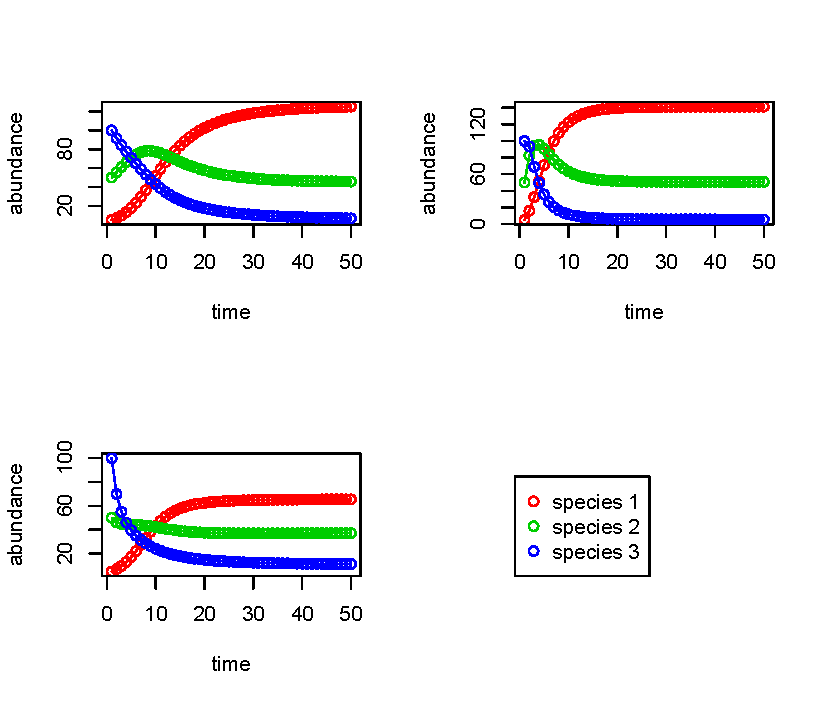
\includegraphics[width=\textwidth]{integrated_multi_competitors.pdf}
\begin{center}
Fig. 1 Three competitors feeding on one constant resource. Initial abundances are $N_1=5$,$N_2=50$,$N_3=100$. For upper left and lower left, $r_1=0.5$,$r_2=0.3$,$r_3=0.1$ while for upper right, all $r$s are scaled up by a factor of 10 ($r_1=5$,$r_2=3$,$r_3=1$). For upper left and upper right, $D_r=0.5$ for all species while for lower left, $D_r=0.1$ for all species.
\end{center}

As Eq. 13 suggests, with $\theta$ and $D_r$ the same for all species, the higher the intrinsic growth rate $r$, the higher the steady state abundance. The difference between upper left and lower left suggests that the smaller the $D_r$ (held same for all species), the more even the steady state abundance distribution or higher chance for existence, a result consistent with MERA I \& II. In addition, comparing upper left and right we can see that, the higher all $r$s are, the more uneven the steady state abundance distribution is, suggesting lower chance for coexistence. Seems that $r$ affects the eventual coexistence pattern in a similar way to $D_r$. Later I will discuss the potential inferences  from this result and how it affects empirical test of the theory.

\subsection{Multiple predators feeding on one prey}

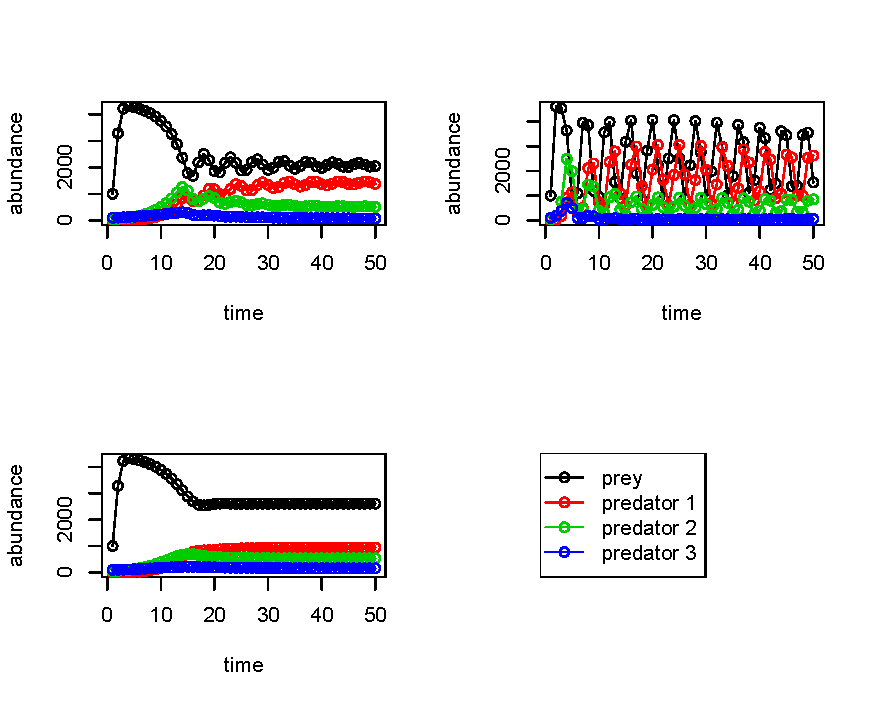
\includegraphics[width=\textwidth]{integrated_multi_predators.pdf}

\begin{center}
The three predators have the same parameter setting as above, for the prey $N_{prey}=1000$, $D_{r,prey}=0$, $\theta_{prey}=1$, the fundamental resource $R_0= 5000$.
\end{center}

We can see that the bigger the magnitude of predator intrinsic growth rates (upper right compared to upper left), the more drastic the oscillation. Smaller predator $D_r$, however, leads to less oscillation in addition to more even steady state abundance distribution.

\section{Discussion}
\subsection{The $D_r$ of a single species community}
Previously in write-up (Oct 16) we have shown that not considering within-species allocation, maximizing resource acquisition macrostates gives a one species growth function slightly slower than predicted by the logistic growth function under the same intrinsic growth rate and carrying capacity (we are talking about the complete redistribution scenario; as you can see, the model developed in this write-up does not assume resource to be fixed in the population once obtained, consistent with the complete scenario). From Eq. 13 we can see that this is actually equivalent to setting $D_r=0$ for the one species. If we change the value of $D_r$, the shape of the growth function varies:

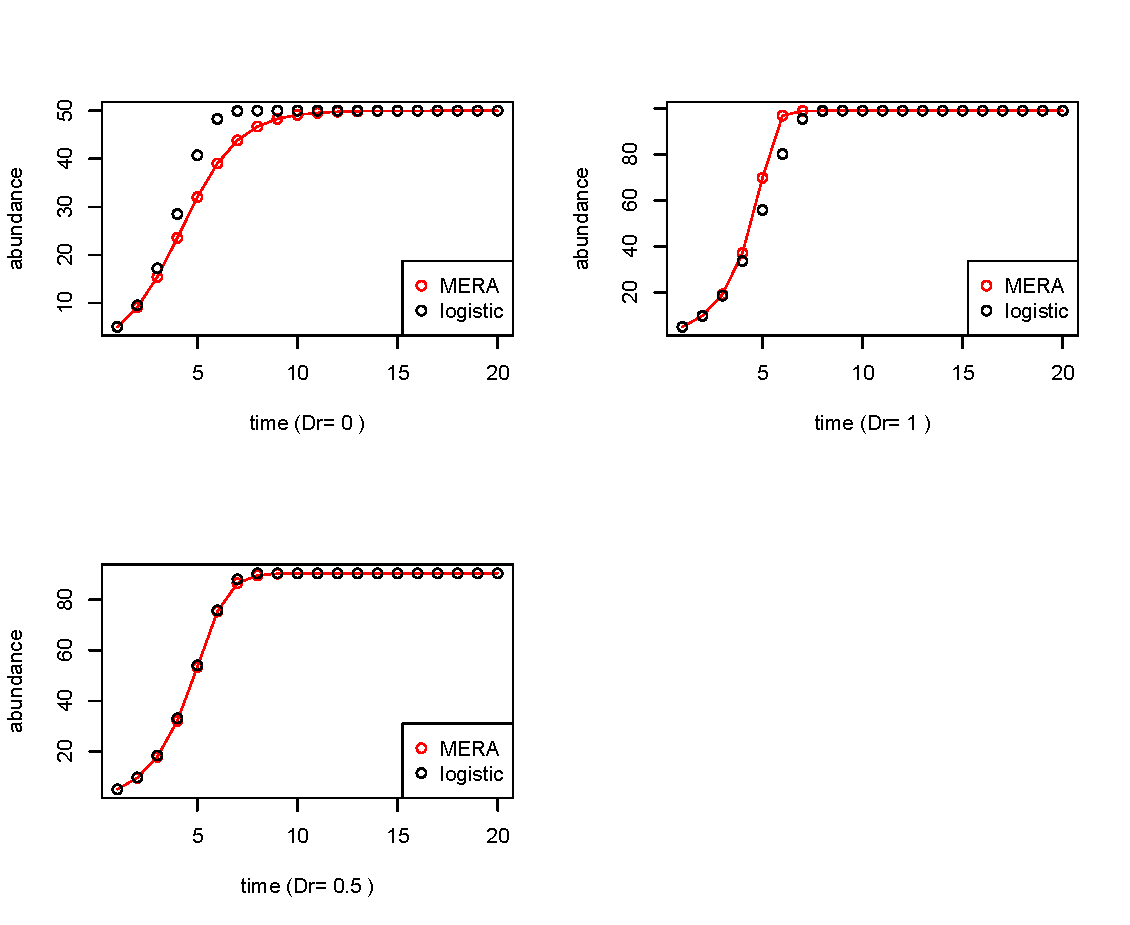
\includegraphics[width=\textwidth]{single_species_Dreffect.pdf}

We can see that as $D_r$ increases, the predicted growth function gets faster and faster compared to the logistic growth function with the same intrinsic growth rate and carrying capacity and the relative steepness between them reverses. When $D_r=1$, the predicted growth function is faster than the logistic growth function; when $D_r=0.5$, they almost completely overlap.

This result has proved that the logistic growth function might be a special case of the model when $D_r=0.5$. In addition to that, I also want to trigger a discussion about what $D_r$ should be in this case, i.e. when there is only one species in the community. 

Based on our current definition and interpretation, $D_r$ is the relative individual distinguishability within the species compared to across species, proxied by the within-species variation (e.g. in certain functional trait) divided by the community variation. Given this, one way to look at the one species case is that since there is only one species, community level variation is the same as within-species variation, therefore $D_r$ should be 1. Then species should always growth faster than the logistic growth function when it is the only species in the community. On the other hand, if we treat the ``unused box'' as the other species (with $D_r=0$), the conclusion might be different: the community level variation has to include the ``unused box'', $D_r$ should be smaller than 1. The actual value of $D_r$ has to be determined by how different the species is from the ``unused box''. If this difference is much bigger than the difference between individuals within the species, then $D_r$ could still be close to 0. In practice, this will probably depend on what the ``unused box'' is, and how different conspecific individuals can be. But it is more natural for me to think that the difference between species and the ``unused box'' ( or ``natural sink''?) is much bigger than the difference between any two individuals within the species, which means $D_r$ is close to 0. Maybe that is not always the case.

The effect of the ``unused box'' gets smaller when there are more species so I don't think it affects the development and test of the theory in multi-species communities. Just for the single-species case it is worth some further thoughts.

\subsection{Oscillation, discretion and time lag}
Time lag might create oscillations, as in discrete L-V.

\subsection{Test the new steady state solution}

Although $r_i$ plays a role in the steady state solution, as long as it scales with $\theta$ following a power-law relationship ($\mbox{log }r \propto \mbox{log }\theta$), $D_{r,i}$ can be estimated by regressing $\mbox{log }N$ against $\mbox{log }\theta$.

The space measurement can still be tested.


\end{document}